\documentclass[12pt]{extreport} % Schriftgröße: 8pt, 9pt, 10pt, 11pt, 12pt, 14pt, 17pt oder 20pt

%% Packages
\usepackage{scrextend}
\usepackage{amssymb}
\usepackage{amsthm}
\usepackage{booktabs}
\usepackage{caption}
\usepackage{subcaption}
\usepackage{chngcntr}
\usepackage{cmap}
\usepackage{color}
\usepackage{csquotes}
\usepackage{enumitem}
\usepackage{float}
\usepackage{graphicx}
\usepackage{hyperref}
\usepackage{ulem}
\usepackage{lmodern}
\usepackage{makeidx}
\usepackage{amsmath}
\usepackage{mathtools}
\usepackage{xpatch}
\usepackage{pgfplots}
\pgfplotsset{compat=1.12}
\usepgfplotslibrary{fillbetween}
\usepackage{amsfonts}
\usetikzlibrary{calc}	
\usetikzlibrary{matrix}	
\usepackage{fancyhdr}
\usepackage{epstopdf}

% Language Setup 
\usepackage[utf8]{inputenc} 
\usepackage[T1]{fontenc} 
\usepackage[ngerman]{babel}

% Options
\makeatletter%%  
  % Linkfarbe, {0,0.35,0.35} für Türkis, {0,0,0} für Schwarz, {1,0,0} für Rot, {0,0,0.85} für Blau
  \definecolor{linkcolor}{rgb}{0,0.35,0.35}
  % Zeilenabstand für bessere Leserlichkeit
  \def\mystretch{1.2} 
  % Publisher definieren
  \newcommand\publishers[1]{\newcommand\@publishers{#1}} 
  % Enumerate im 1. Level: \alph für a), b), ...
  \renewcommand{\labelenumi}{\alph{enumi})} 
  % Enumerate im 2. Level: \roman für (i), (ii), ...
  \renewcommand{\labelenumii}{(\roman{enumii})}
  % Zeileneinrückung am Anfang des Absatzes
  \setlength{\parindent}{0pt} 
  % Für das Proof-Environment: 'Beweis:' anstatt 'Beweis.'
  \xpatchcmd{\proof}{\@addpunct{.}}{\@addpunct{:}}{}{} 
  % Nummerierung der Bilder, z.B.: Abbildung 4.1
  \@ifundefined{thechapter}{}{\def\thefigure{\thechapter.\arabic{figure}}} 
  % Chapter-Nummerierung beginnen bei (0):
  \setcounter{chapter}{0}
  % Chapter-Nummerierung
  \renewcommand\thechapter{\Roman{chapter}}
\makeatother%

% Meta Setup 
\title{Globale Optimierung - Sonderübung III}
\author{Kostorz, Belica}
\date{Sommersemester 2017}
\publishers{Karlsruher Institut für Technologie}

\fancypagestyle{firststyle}
{
   \fancyhf[C]{\small Globale Optimierung - Sonderübung III ~\\ Nadine Kostorz (1972005), Leon Talenberg (1957966), Martin Belica (1775706)}
   \fancyfoot[C]{}
}

%% Math. Definitiones
\newcommand{\C}{\mathbb{C}}
\newcommand{\N}{\mathbb{N}}
\newcommand{\Q}{\mathbb{Q}}
\newcommand{\R}{\mathbb{R}}
\newcommand{\Z}{\mathbb{Z}}
\newcommand{\DO}[1]{\mathcal{D}\left( {#1} \right)}
\newcommand{\RO}[1]{\mathcal{R}\left( {#1} \right)}

%% Template
\makeatletter%
\DeclareUnicodeCharacter{00A0}{ } \pgfplotsset{compat=1.7} \hypersetup{colorlinks,breaklinks, urlcolor=linkcolor, linkcolor=linkcolor, pdftitle=\@title, pdfauthor=\@author, pdfsubject=\@title, pdfcreator=\@publishers}\DeclareOption*{\PassOptionsToClass{\CurrentOption}{report}} \ProcessOptions \def\baselinestretch{\mystretch} \setlength{\oddsidemargin}{0.125in} \setlength{\evensidemargin}{0.125in} \setlength{\topmargin}{0.5in} \setlength{\textwidth}{6.25in} \setlength{\textheight}{8in} \addtolength{\topmargin}{-\headheight} \addtolength{\topmargin}{-\headsep} \def\pulldownheader{ \addtolength{\topmargin}{\headheight} \addtolength{\topmargin}{\headsep} \addtolength{\textheight}{-\headheight} \addtolength{\textheight}{-\headsep} } \def\pullupfooter{ \addtolength{\textheight}{-\footskip} } \def\ps@headings{\let\@mkboth\markboth \def\@oddfoot{} \def\@evenfoot{} \def\@oddhead{\hbox {}\sl \rightmark \hfil \rm\thepage} \def\chaptermark##1{\markright {\uppercase{\ifnum \c@secnumdepth >\m@ne \@chapapp\ \thechapter. \ \fi ##1}}} \pulldownheader } \def\ps@myheadings{\let\@mkboth\@gobbletwo \def\@oddfoot{} \def\@evenfoot{} \def\sectionmark##1{} \def\subsectionmark##1{}  \def\@evenhead{\rm \thepage\hfil\sl\leftmark\hbox {}} \def\@oddhead{\hbox{}\sl\rightmark \hfil \rm\thepage} \pulldownheader }	\def\chapter{\cleardoublepage  \thispagestyle{plain} \global\@topnum\z@ \@afterindentfalse \secdef\@chapter\@schapter} \def\@makeschapterhead#1{ {\parindent \z@ \raggedright \normalfont \interlinepenalty\@M \Huge \bfseries  #1\par\nobreak \vskip 40\p@ }} \newcommand{\indexsection}{chapter} \patchcmd{\@makechapterhead}{\vspace*{50\p@}}{}{}{}\def\Xint#1{\mathchoice
    {\XXint\displaystyle\textstyle{#1}} {\XXint\textstyle\scriptstyle{#1}} {\XXint\scriptstyle\scriptscriptstyle{#1}} {\XXint\scriptscriptstyle\scriptscriptstyle{#1}} \!\int} \def\XXint#1#2#3{{\setbox0=\hbox{$#1{#2#3}{\int}$} \vcenter{\hbox{$#2#3$}}\kern-.5\wd0}} \def\dashint{\Xint-} \def\Yint#1{\mathchoice {\YYint\displaystyle\textstyle{#1}} {\YYYint\textstyle\scriptscriptstyle{#1}} {}{} \!\int} \def\YYint#1#2#3{{\setbox0=\hbox{$#1{#2#3}{\int}$} \lower1ex\hbox{$#2#3$}\kern-.46\wd0}} \def\YYYint#1#2#3{{\setbox0=\hbox{$#1{#2#3}{\int}$}  \lower0.35ex\hbox{$#2#3$}\kern-.48\wd0}} \def\lowdashint{\Yint-} \def\Zint#1{\mathchoice {\ZZint\displaystyle\textstyle{#1}}{\ZZZint\textstyle\scriptscriptstyle{#1}} {}{} \!\int} \def\ZZint#1#2#3{{\setbox0=\hbox{$#1{#2#3}{\int}$}\raise1.15ex\hbox{$#2#3$}\kern-.57\wd0}} \def\ZZZint#1#2#3{{\setbox0=\hbox{$#1{#2#3}{\int}$} \raise0.85ex\hbox{$#2#3$}\kern-.53\wd0}} \def\highdashint{\Zint-} \DeclareRobustCommand*{\onlyattoc}[1]{} \newcommand*{\activateonlyattoc}{ \DeclareRobustCommand*{\onlyattoc}[1]{##1} } \AtBeginDocument{\addtocontents{toc} {\protect\activateonlyattoc}} \newcommand{\RightArrow}{\xRightarrow[]{ ~ ~ }} \newcommand{\LeftArrow}{\xLeftarrow[]{ ~ ~ }} \newcommand{\rightArrow}{\xrightarrow[]{ ~ ~ }} \newcommand{\leftArrow}{\xleftarrow[]{ ~ ~ }}
	% Titlepage
	\def\maketitle{ \begin{titlepage} 
			~\vspace{3cm} 
		\begin{center} {\Huge \@title} \end{center} 
	 		\vspace*{1cm} 
	 	\begin{center} {\large \@author} \end{center} 
	 	\vspace*{-0.5cm}
	 	\begin{center} \@date \end{center} 
	 		\vspace*{7cm} 
	 	\begin{center} \@publishers \end{center} 
	 		\vfill 
	\end{titlepage} }
\makeatother%

% Create Index
\makeindex 

\begin{document}

\thispagestyle{empty}
\pagenumbering{arabic}\thispagestyle{firststyle}

\subsubsection*{Aufgabe 1}

Für eine Menge $M \subseteq \R^n$ bezeichnet 
	$$ d(X) \coloneqq \sup_{x,y \in M} \| x - y \|_2 $$
den Durchmesser von $M$. Zeigen Sie, dass der Durchmesser einer Box $X$ mit ihrer Boxweite übereinstimmt.

\begin{proof}
	Sei $N \coloneqq \{1, \dotsc, n\}$. Es gilt für die Boxweite $w$:
	$$ w(X) = \| \overline{x} - \underline{x} \|_2. $$ 
	Da $Z \coloneqq \{ \overline{x}, \underline{x} \} \subseteq X$, gilt damit
	$$ d(X) = \sup_{x,y \in X} \| x - y \|_2 \geq \sup_{x,y \in Z } \| x - y \|_2 = w(X), $$
	d.h. um die Behauptung zu zeigen bleibt $w(X) \geq d(X)$ offen. Angenommen dies gilt nicht, d.h.
	\begin{align*}
		 w(X) < d(X). \tag*{$(*)$}
	\end{align*}
	Da die Box $X$ aufgrund der Definition abgeschlossen ist, existieren $\tilde{x}, \tilde{y} \in X$, sodass
	$$ d(X) = \sup_{x,y \in M} \| x - y \|_2 = \| \tilde{x} - \tilde{y} \|_2 $$
	Damit folgt aus $(*)$:
	 $$ \| \overline{x} - \underline{x} \|_2 < \| \tilde{x} - \tilde{y} \|_2, $$
	 was äquivalent ist zu
	 $$ \sum_{i \in N} | \overline{x}_i - \underline{x}_i |^2 < \sum_{ i \in N} | \tilde{x}_i - \tilde{y}_i |^2. $$
	Damit diese Ungleichung erfüllt ist, muss mindestens für einen Summanden $j$ 
	\begin{align*}
		| \overline{x}_j - \underline{x}_j | <  | \tilde{x}_j - \tilde{y}_j | \tag*{$(**)$}
	\end{align*} 
	gelten. Sei nun $d_j \coloneqq | \overline{x}_j - \underline{x}_j |$ die Breite und $m_j \coloneqq \frac{1}{2} \left( \overline{x}_j - \underline{x}_j \right)$ die Mitte dieses eindimensionalen Intervalls $I_j = \left[ \underline{x}_j, \overline{x}_j \right]$. Nach Konstruktion gilt $\tilde{x}, \tilde{y} \in X$, was insbesondere $\tilde{x}_j, \tilde{y}_j \in I_j$ impliziert. Nach $(**)$ folgt mit der Abgeschlossenheit von $I_j$ damit
	\begin{align*}
		d_j & = \left| \overline{x}_j - \underline{x}_j \right| \\
			& <  \left| \tilde{x}_j - \tilde{y}_j \right| \\
			& \leq \left| \tilde{x}_j - m_j \right| + \left| m_j - \tilde{y}_j \right| \\
			& \leq \sup_{\overline{z} \in I_j} \left| \overline{z} - m_j \right| + \sup_{\underline{z} \in I_j} \left| m_j - \underline{z} \right|  \\ 
			& =  \frac{1}{2} d_j + \frac{1}{2} d_j,
	\end{align*}
	was einen Widerspruch darstellt, und somit gilt $w(X) = d(X)$ .
\end{proof}

\newpage

\subsubsection*{Aufgabe 2}

\begin{enumerate}
	\item Implementieren Sie eine Funktion $interval\_hull(A)$, die einer beschränkten Menge reeller Zahlen $A \coloneqq [a_1, . . . , a_n]$ die Intervallhülle $[\inf A, \sup A]$ zuordnet.
		\begin{proof} ~\
			\begin{figure*}[h!] \centering
				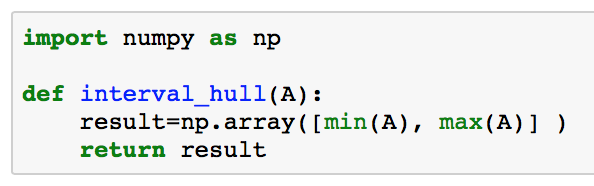
\includegraphics[scale=0.75]{img/su2ii-i}
			\end{figure*}
		\end{proof}
	\item Implementieren Sie die Intervall-Grundrechenarten (vgl. Skript S. 126 - 129) für die Addition, Subtraktion und Multiplikation zweier Intervalle $X, Y \in \mathbb{IR}$ in den Funktionen $interval\_add(X,Y)$, $interval\_subtract(X,Y)$ und   $interval\_multiply(X,Y)$.
		\begin{proof} ~\
			\begin{figure*}[h!] \centering
				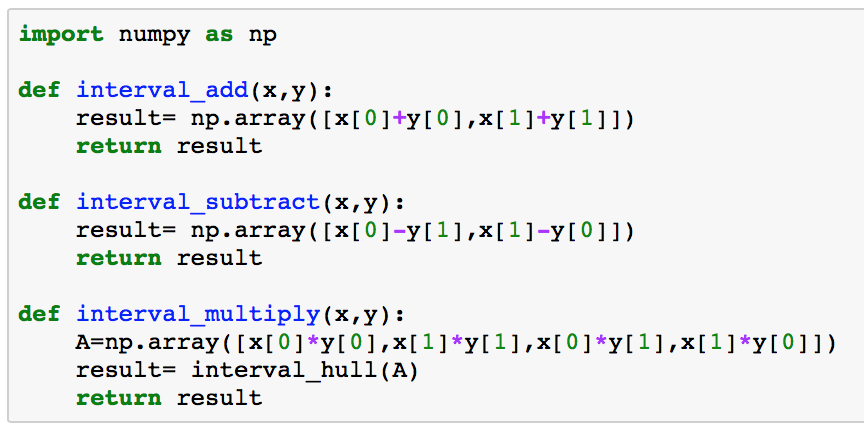
\includegraphics[scale=0.75]{img/su2ii-ii}
			\end{figure*}
		\end{proof} \newpage
	\item Implementieren Sie eine Funktion, die den Durchmesser einer eindimensionalen Box $X \in \mathbb{IR}$ berechnet.
		\begin{proof} ~\
			\begin{figure*}[h!] \centering
				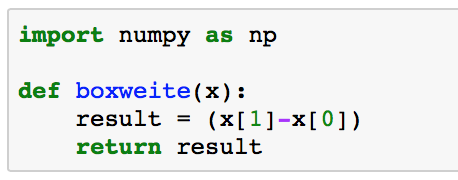
\includegraphics[scale=0.75]{img/su2ii-iii}
			\end{figure*}
		\end{proof}
	\item Implementieren Sie eine Funktion, die den Boxmittelpunkt einer eindimensionalen Box $X \in \mathbb{IR}$ berechnet.
		\begin{proof} ~\
			\begin{figure*}[h!] \centering
				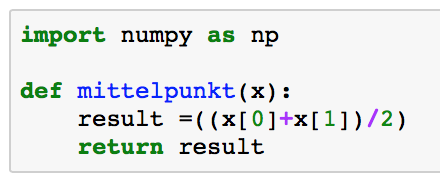
\includegraphics[scale=0.75]{img/su2ii-iv}
			\end{figure*}
		\end{proof}
\end{enumerate}

\newpage

\subsubsection*{Aufgabe  3}

Gegeben sei die Funktion $f \colon \R \rightarrow \R$, $f(x) \coloneqq x - x^2 = x - x \cdot x = x \cdot \left( 1 - x \right)$ und die intervallwertigen Funktionen
	$$ F_1 \colon \mathbb{IR} \rightarrow \mathbb{IR}, ~ F_1(X) = X - X X, \quad F_2 \colon \mathbb{IR} \rightarrow \mathbb{IR}, ~ F_2(X) = X(1- X) $$
\begin{enumerate}
	\item Zeigen Sie, dass $F_1$, als auch $F_2$ eine natürliche Intervallerweiterung von $f$ ist.
		\begin{proof} 
			Zunächst gilt, dass $f(x)$ als Komposition von Grundrechenarten nach Definition 3.3.2 eine faktorisierbare Funktion ist. Mit 
			$$ F_1(X) = X-XX = X-X^2 = f(x) $$
			gilt nach Definition 3.3.4, dass $F_1$ die natürliche Intervallerweiterung von $f$ ist. Analog gilt mit 
			$$ F_2(X)=X(1-X)=X-XX=X-X^2=f(X) $$
			nach Definition 3.3.4, dass $F_2$ die natürliche Intervallerweiterung von $f$ ist.
		\end{proof}
	\item Bestimmen Sie durch geschickte Fallunterscheidung
		$$ F_3 \colon \mathbb{IR} \rightarrow \mathbb{IR}, ~ F_3(X) = \operatorname{bild}(f, X) $$
		für ein beliebiges Intervall $X \subseteq \mathbb{IR}$ explizit. Zeigen Sie, dass die von Ihnen definierte intervallwertige Funktion $F_3$ für ein beliebiges Intervall tatsächlich die Bildmenge $\operatorname{bild}(f, X)$ liefert.
		\begin{proof}
			Die Funktion $f$ ist als Polynom in $C^1(\R)$ und das Bild somit ein  Intevrall. Außerdem ist wegen 
				$$ f'(x) = 1 - 2x $$ 
			die Funktion $f$ 
			\begin{itemize}
				\item monoton steigend für $x < \frac{1}{2}$, und
				\item monoton fallend für $x > \frac{1}{2}$.
			\end{itemize}
			Damit ist für $X \subseteq \left(-\infty, \frac{1}{2} \right)$ oder $X \subseteq \left(\frac{1}{2}, \infty \right)$ das Bild von $f$ unter $X$, ein Intevrall dessen Grenzen durch die Grenzen von $X$ unter $f$ gegeben ist. Somit ist
			\begin{itemize}
				\item für $\overline{x} < 1/2$ (d.h. $X \subseteq \left(-\infty, \frac{1}{2} \right)$) $f(\underline{x}) < f(\overline{x})$, d.h.:
					$$ \operatorname{bild}(f,X) = \left[f(\underline{x}), f(\overline{x}) \right]; $$
				\item für $\underline{x} >1/2$ (d.h. $X \subseteq \left(\frac{1}{2}, \infty \right)$) $f(\overline{x}) < f(\underline{x})$, d.h.:
					$$ \operatorname{bild}(f,X) = \left[f(\overline{x}), f(\underline{x})\right]; $$
			\end{itemize}
			Ist hingegen $\frac{1}{2} \in X$, so folgt wegen
				$$ f''(x) = 2 < 0 $$
			 und der Monotonie auf den Teilintervallen, dass $f \left( \frac{1}{2} \right) = \frac{1}{4}$ die Obergrenze der Bildmenge ist. Die Untergrenze ergibt sich aus der Vereinigung der Bildmenge des Intervalls links von $\frac{1}{2}$, auf dem $f$ monoton steigend ist, und rechts von $\frac{1}{2}$, auf dem $f$ monoton fallend ist. Nach Obigem folgt somit:
					$$ \operatorname{bild}(f,X) = \left[ \min \left\{ f(\underline{x}), f(\overline{x}) \right\}, f \left( \frac{1}{2} \right) \right] $$
		\end{proof}
	\item Implementieren Sie die intervallwertigen Funktionen $F_1$, $F_2$ und $F_3$.
		\begin{proof} ~\
			\begin{figure*}[h!] \centering
				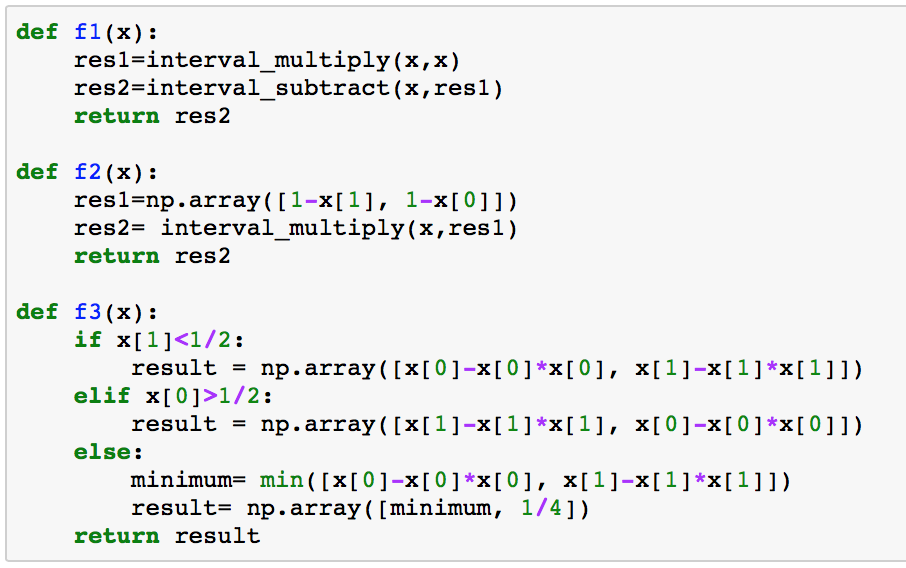
\includegraphics[scale=0.45]{img/su2iii-iii}
			\end{figure*}
		\end{proof}   \newpage
	\item Berechnen Sie Boxweite und Boxmittelpunkt von $Y_i = F_i(X(\epsilon))$, $i = 1,2,3$, für das Intervall $X = [-10, -10 + \epsilon]$ für $\epsilon \in \{ 0.1, 0.2, \dotsc, 30\}$. Erstellen Sie zwei Plots, die Boxmittelpunkt und Boxweite der Funktionen über der Boxweite von $X(\epsilon)$ darstellen.
		\begin{proof} ~\
			\begin{figure*}[h!] \centering
				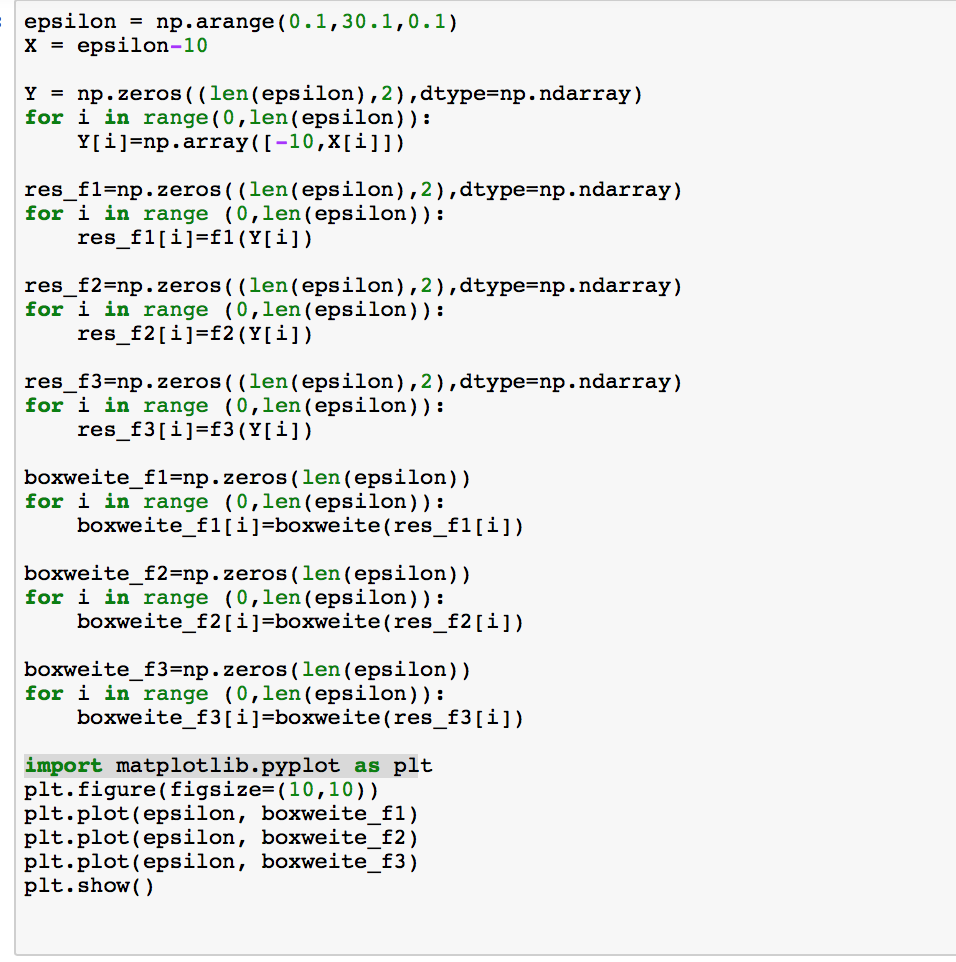
\includegraphics[scale=0.45]{img/su2iii-iiii-11}
				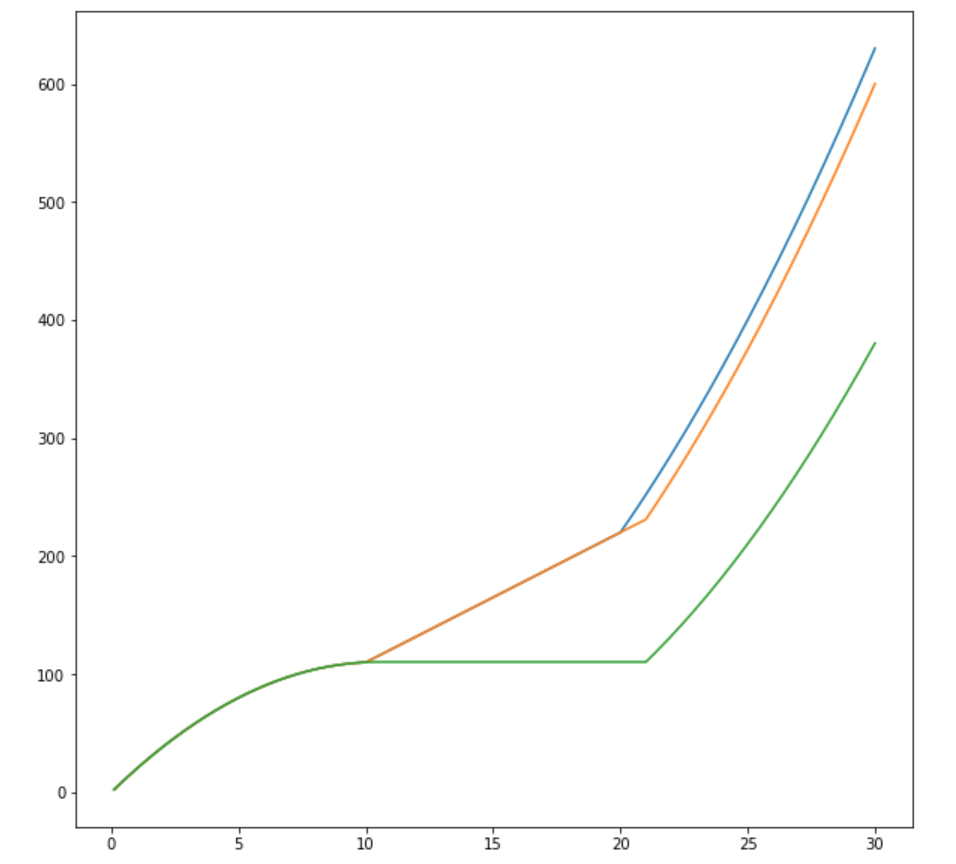
\includegraphics[scale=0.45]{img/su2iii-iiii-12}
			\end{figure*}
		\end{proof}
	\item Erklären Sie: Woraus resultiert das Verhalten von Boxweite und Boxmittelpunkt für $F_3(X(\epsilon))$? Untersuchen Sie hierzu genau das Verhalten von Unter- und Obergrenze von $F_3(X(\epsilon))$ für $\epsilon \in [0, 30]$.Welche der beiden Funktionen $F_1$, $F_2$ approximiert $\operatorname{bild}(f, X)$ besser? Warum?
		\begin{proof}
			Verhalten der Boxweite: 
			\begin{itemize}
				\item für $\epsilon < 10.5$ : Untergrenze bleibt konstant bei $f(-10)$, Obergrenze steigt degressiv mit Funktionsgraph $f(-10+\epsilon)$ bis Max=1/4 $\Rightarrow$ Boxweite zeichnet degressiven Verlauf
				\item für $10.5 \leq \epsilon \leq 21$ bleiben Untergrenze  und Obergrenze von $F_3(X(\epsilon))$ konstant und damit auch die Boxweite
				\item für $\epsilon>21$ Obergrenze konst. (=1/4) und Untergrenze sinkt mit Funktionsgraph und damit steigt die Boxweite weiter degressiv an bis $\epsilon=30$
			\end{itemize}
			Verhalten des Boxmittelpunktes:
			\begin{itemize}
				\item für $\epsilon <10.5$ : Untergrenze bleibt konst. bei $f(-10)$, Obergrenze steigt degressiv mit Funktionsgraph $f(-10+\epsilon)$ bis Max=1/4 $\Rightarrow$ Boxmittelpunkt zeichnet degressiv steigenden Verlauf
				\item für $10.5 \leq \epsilon \leq 21$ bleiben Untergrenze  und Obergrenze von $F_3(X(\epsilon))$ konstant und damit auch der Boxmittelpunkt
				\item für $\epsilon>21$ Obergrenze konst. (=1/4) und Untergrenze sinkt mit Funktionsgraph $\Rightarrow$ der Boxmittelpunkt verschiebt sich wieder nach unten bis $\epsilon=30$
			\end{itemize}
			$F_2(X)$ approximiert die Bildmenge $\operatorname{bild}(f,X)$ am Besten, da sie sie im Sinne des Abhängigketseffektes am wenigsten verzerrt. Ihre Funktionsvorschrift $F2(X)=X(1-X)$ enthält offensichtlich nur 2 mal das Intervall X, $F_3(X)=X-XX$ dagegen 3 mal.
		\end{proof}
\end{enumerate}

\end{document}